
%!TEX root = ../thesis.tex
%*******************************************************************************
%****************************** Third Chapter **********************************
%*******************************************************************************
\chapter{Calibration}

% **************************** Define Graphics Path **************************
\ifpdf
    \graphicspath{{Chapter7/Figs/Raster/}{Chapter7/Figs/PDF/}{Chapter7/Figs/}}
\else
    \graphicspath{{Chapter7/Figs/Vector/}{Chapter7/Figs/}}
\fi

%********************************** %Opening  **************************************
Calibration is a crucial step to investigate and correct the detector response to the deposited energy to produce signals, such as charge collected on anode wires or photoelectrons seen by PMTs.
Chapter \ref{Chapter3} provides an overview of the detector effects of a LArTPC that can smear out the signals as they propagate toward detection.
Earlier LArTPC experiments like MicroBooNE \cite{uboone_calib, ubooneEtime}, ArgoNeuT \cite{argoneut_recomb}, and ICARUS \cite{icarus_recomb, GrayDiffusion} have demonstrated the particular importance of calibrating charge signals on anode wires, improving the spatial, temporal, as well as energy resolution to achieve exceptional imaging capability.

Two simulation studies within the scope of charge calibration are presented in this chapter.
The first study is presented in Sec. \ref{sec7:etime}, focusing on electron lifetime measurement.
Sec. \ref{sec7:etime_procedure} outlines a measurement procedure using an anode-to-cathode crossing cosmic track sample, whilst Sec. \ref{sec7:etime_bias} identifies detector effects that can introduce biases in the lifetime measurement.
Improvements and updates on the procedure are summarised in Sec. \ref{sec7:etime_remark}.
The second study is provided in Sec. \ref{sec7:delta}, assessing the impacts of delta ray fluctuation on recombination to have a better understanding of the simulation framework for this phenomenon.
Sec. \ref{sec:simDeltaRay} details the simulation framework of delta rays and recombination.
Sec. \ref{sec:impactDeltaRayMag} and \ref{sec:impactDeltaRaySmear} describe the impacts of delta rays on the magnitude and smearing of recombination respectively, while Sec. \ref{sec:impactStepLimit} examines the length scale of the simulation framework.
Finally, Sec. \ref{sec:concludeDeltaRay} provides suggestions for measurements that can carried out at SBND to improve and build toward a data-driven recombination model.

\newpage
%********************************** %First Section  **************************************
\section{Electron Lifetime Measurement}
\label{sec7:etime}
% purity monitoring by SBND + calibration
Drifting electrons can be captured by electronegative impurities present in LAr, as previously described in Sec. \ref{sec:edrift}.
At SBND, three purity monitors were installed, two internal to the cryostat and one external, to provide quick and real-time monitoring of the LAr purity.
Meanwhile, calibration will require a dedicated procedure to model electron attenuation using the charge collected by the wires.
Electron attenuation is modelled as an exponential suppression as Eq. \ref{eq:etime}, where $\tau$ is the electron lifetime constant to be measured.
The lifetime constant must be accurately measured, to recover the original charge deposition before drifting to the wires.

The MicroBooNE experiment has previously used anode-to-cathode-crossing cosmic tracks for electron lifetime measurement \cite{uboone_calib}.
These tracks enter the detector from either the cathode or anode and exit through the opposite plane.
Since they fully traverse the whole drift distance of the TPC,   a good sample to study the measured charge per unit length $dQ/dx$ dependency on the drift distance.
For the calibration run of SBND in the summer of 2024, a calibration trigger will be deployed to tag tracks of this topology and produce a dedicated sample for electron lifetime measurement.
Within the scope of this study, a sample of crossing cosmic tracks was simulated to perform the lifetime measurement.

The study aims to develop a procedure to measure electron lifetime and investigate detector effects that can introduce biases on the lifetime, such as diffusion and Space Charge Effect (SCE).
The procedure for electron lifetime measurement is outlined in Sec. \ref{sec7:etime_procedure}, followed by Sec. \ref{sec7:etime_bias} describing biases in lifetime measurement due to detector effect
s.
Finally, Sec. \ref{sec7:etime_remark} provides recent updates and improvements to carry on the electron lifetime measurement with data.

\subsection{Procedure}
\label{sec7:etime_procedure}

The electron lifetime measurement requires information on the measured charge per unit length $dQ/dx$ and the respective drift time $t_{drift}$ of that charge cluster collected on the wire.
The charge reconstruction follows the signal processing workflow described in Chapter \ref{Chapter6}, whilst additional calculation is required to deduce the drift time.     
The drift time is defined as follows                                                                                          
\begin{equation}
        t_{drift} = \frac{x}{v_{d}}
\end{equation}
where $x$ is the drift coordinate of the charge deposition relative to the APA and $v_{d}$ is the drift velocity.
For the TPCs of SBND, the drift velocity is 0.1563 cm/$\mu$s at an electric field of 0.5 kV/cm and liquid argon temperature of 88.4 K.
The drift time can be calculated using the measured time $t_{m}$ recorded by the TPC readout when a charge cluster arrives at a wire, which is defined as \cite{pandora_protodune}
\begin{equation}
\label{eq:t0}
        t_{m} = t_{0} - t_{trigger} + t_{drift} 
\end{equation}
where $t_{0}$ is the time when the particle enters the detector and $t_{trigger}$ is the time when the TPC readout is triggered.
For a beam neutrino that triggers the TPC readout, the readout is configured to align with when the beam arrives at the detector hall such that $t_{trigger} = t_{0}$ by definition.
Meanwhile, a cosmic track can occur anytime within the readout window, and the time when it enters the detector $t_{0}$ is ambiguous.

A \textit{stitching} process was developed by the ProtoDUNE and Pandora collaboration to resolve the ambiguous $t_{0}$ of cosmic tracks that cross the cathode \cite{pandora_protodune}.
This medthod can be applied to any LArTPC experiments that have two TPCs sharing the same cathode.
Fig. \ref{fig:cosmic_stitch} depicts the \textit{stitching} process.
Two cosmic track segments, in red and blue lines, were reconstructed under an initial assumption of $t_{0} = 0$, and thus, they appear at the wrong positions in both drift volumes.
The reconstruction algorithm then shifts the drift coordinate in each TPC by an equal and opposite amount until the two segments are \textit{stitched} at the cathode, in black line, recovering 
the correct $t_{0}$.                                                                                                                                                                                   
This method has been implemented in the reconstruction workflow of SBND, and it was applied to reconstruct the sample of anode-to-cathode-crossing tracks in this study.
%Once $t_{0}$ is determined, the drift time can then be calculated using Eq. \ref{eq:t0}. 

\begin{figure}[htbp!] 
\centering    
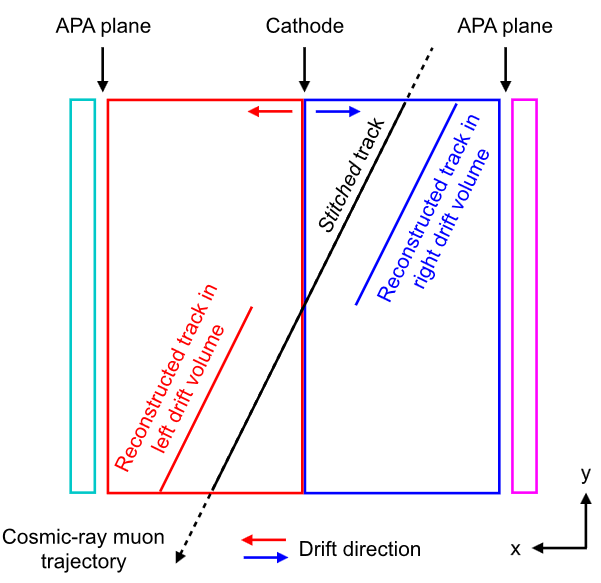
\includegraphics[width=0.5\textwidth]{cosmic_stitch}
\caption[cosmic_stitch]{
	Diagram depicting the \textit{cathode stictching} process to determine the $t_{0}$ of cathode-crossing tracks.
	Fig. from \cite{pandora_protodune}.
}
\label{fig:cosmic_stitch}
\end{figure}

One can then construct the 1D profile of $dQ/dx$ for the charge collected on the collection plane for a given bin of drift time as shown in Fig. \ref{fig:dqdxMPV}, for an example $dQ/dx$ profile of the drift
 time bin from 0.925 to 0.95 ms.                                                                                                                                                                       
A Landau convoluted with a Gaussian distribution \cite{Passage} is fitted to the profile to extract the Most Probable Value (MPV) of $dQ/dx$.                                 
The MPV $dQ/dx$ is then plotted with respect to its drift time as shown in Fig. \ref{fig:etime_tpc}, for TPC 0 and 1 of SBND.                                                                          
Bins of drift time less than 0.25 ms and larger than 1.15 ms are excluded due to the close proximity to the anode and cathode respectively, which can introduce boundary effects to the charge clusters
.                                                                                                                                                                                                      
The MPV $dQ/dx$ distribution is fitted with Eq. \ref{eq:etime} to determine the electron lifetime constant.                                                                                            
The sample input to Fig. \ref{fig:etime_tpc} was simulated with a lifetime of 10 ms and no detector effects enabled to validate the procedure.                                       
The measured lifetimes of 10.12 and 10.40 ms, for TPC 0 and 1 respectively, show a good agreement with simulation. 
\begin{figure}[htbp!] 
\centering    
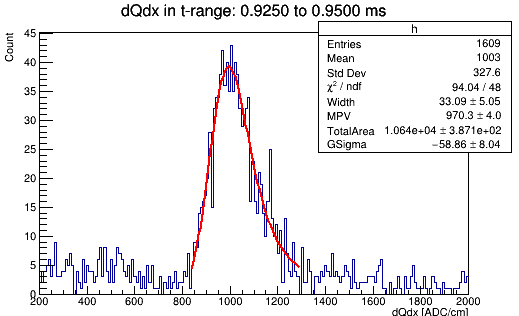
\includegraphics[width=0.55\textwidth]{dqdxMPV}
\caption[dqdxMPV]{
$dQ/dx$ profile for the drift time from 0.925 to 0.95 ms, fitted with a Landau convoluted with Gaussian distribution to determine the MPV $dQ/dx$.
}
\label{fig:dqdxMPV}
\end{figure}
\begin{figure}[htbp!]
        \centering
        \begin{subfigure}[b]{0.495\textwidth}
            \centering
            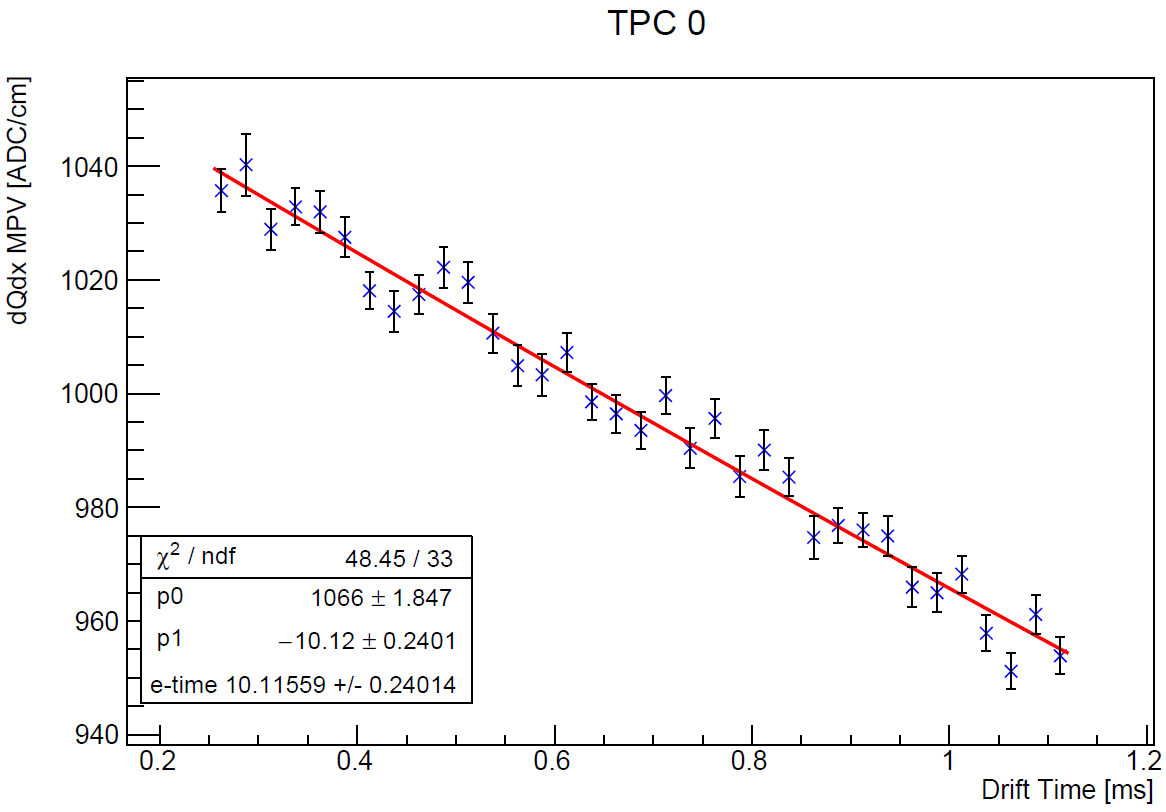
\includegraphics[width=\textwidth]{etime_tpc0}
            %\caption{}%
            %\label{}
        \end{subfigure}
        \hfill
        \begin{subfigure}[b]{0.495\textwidth}  
            \centering 
            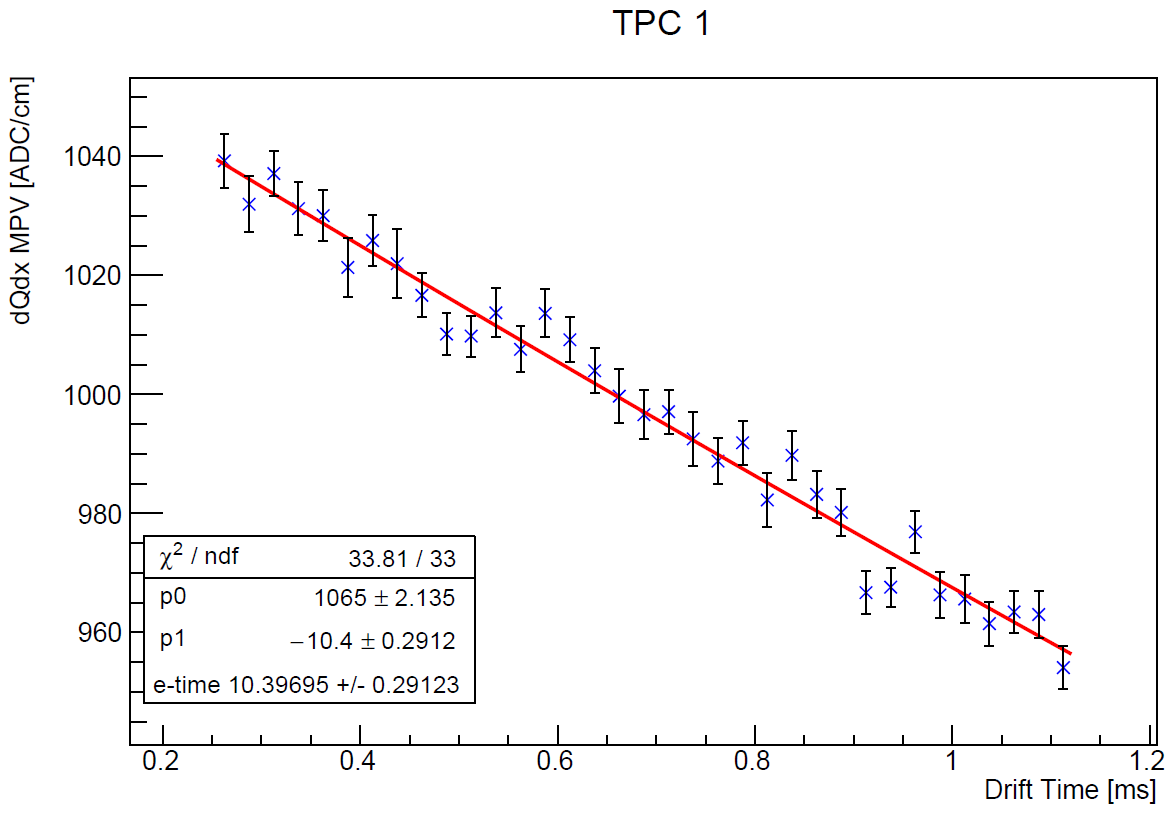
\includegraphics[width=\textwidth]{etime_tpc1}
            %\caption{}%
            %\label{}
        \end{subfigure}
        \caption[etime_tpc]{MPV $dQ/dx$ as a function drift time, fitted with an exponential decay function to determine the electron lifetime constant.}
        \label{fig:etime_tpc}
\end{figure}

\subsection{Bias Study From Diffusion and Space Charge Effects}
\label{sec7:etime_bias}

Some detector effects can introduce biases to the electron lifetime measurement, specifically those that can influence the propagation path of drifting electrons such as diffusion and SCE, as detailed
 in Sec. \ref{sec3:diffusion}.
Diffusion can smear both spatial and temporal resolution of the drifting electrons, and consequently the measured time of charge collected on the wires.
Meanwhile, SCE impacts both the amplitude of the charge collected on the wire as well as the temporal and spatial resolution of the drifting coordinates due to electric field distortion.
This study aims to understand how individual effect introduces biases to the measured electron lifetime.
Dedicated samples were simulated, with neither nor only one detector effect enabled at a time, and electron lifetime was measured for each sample.

\begin{figure}[bp!] 
\centering    
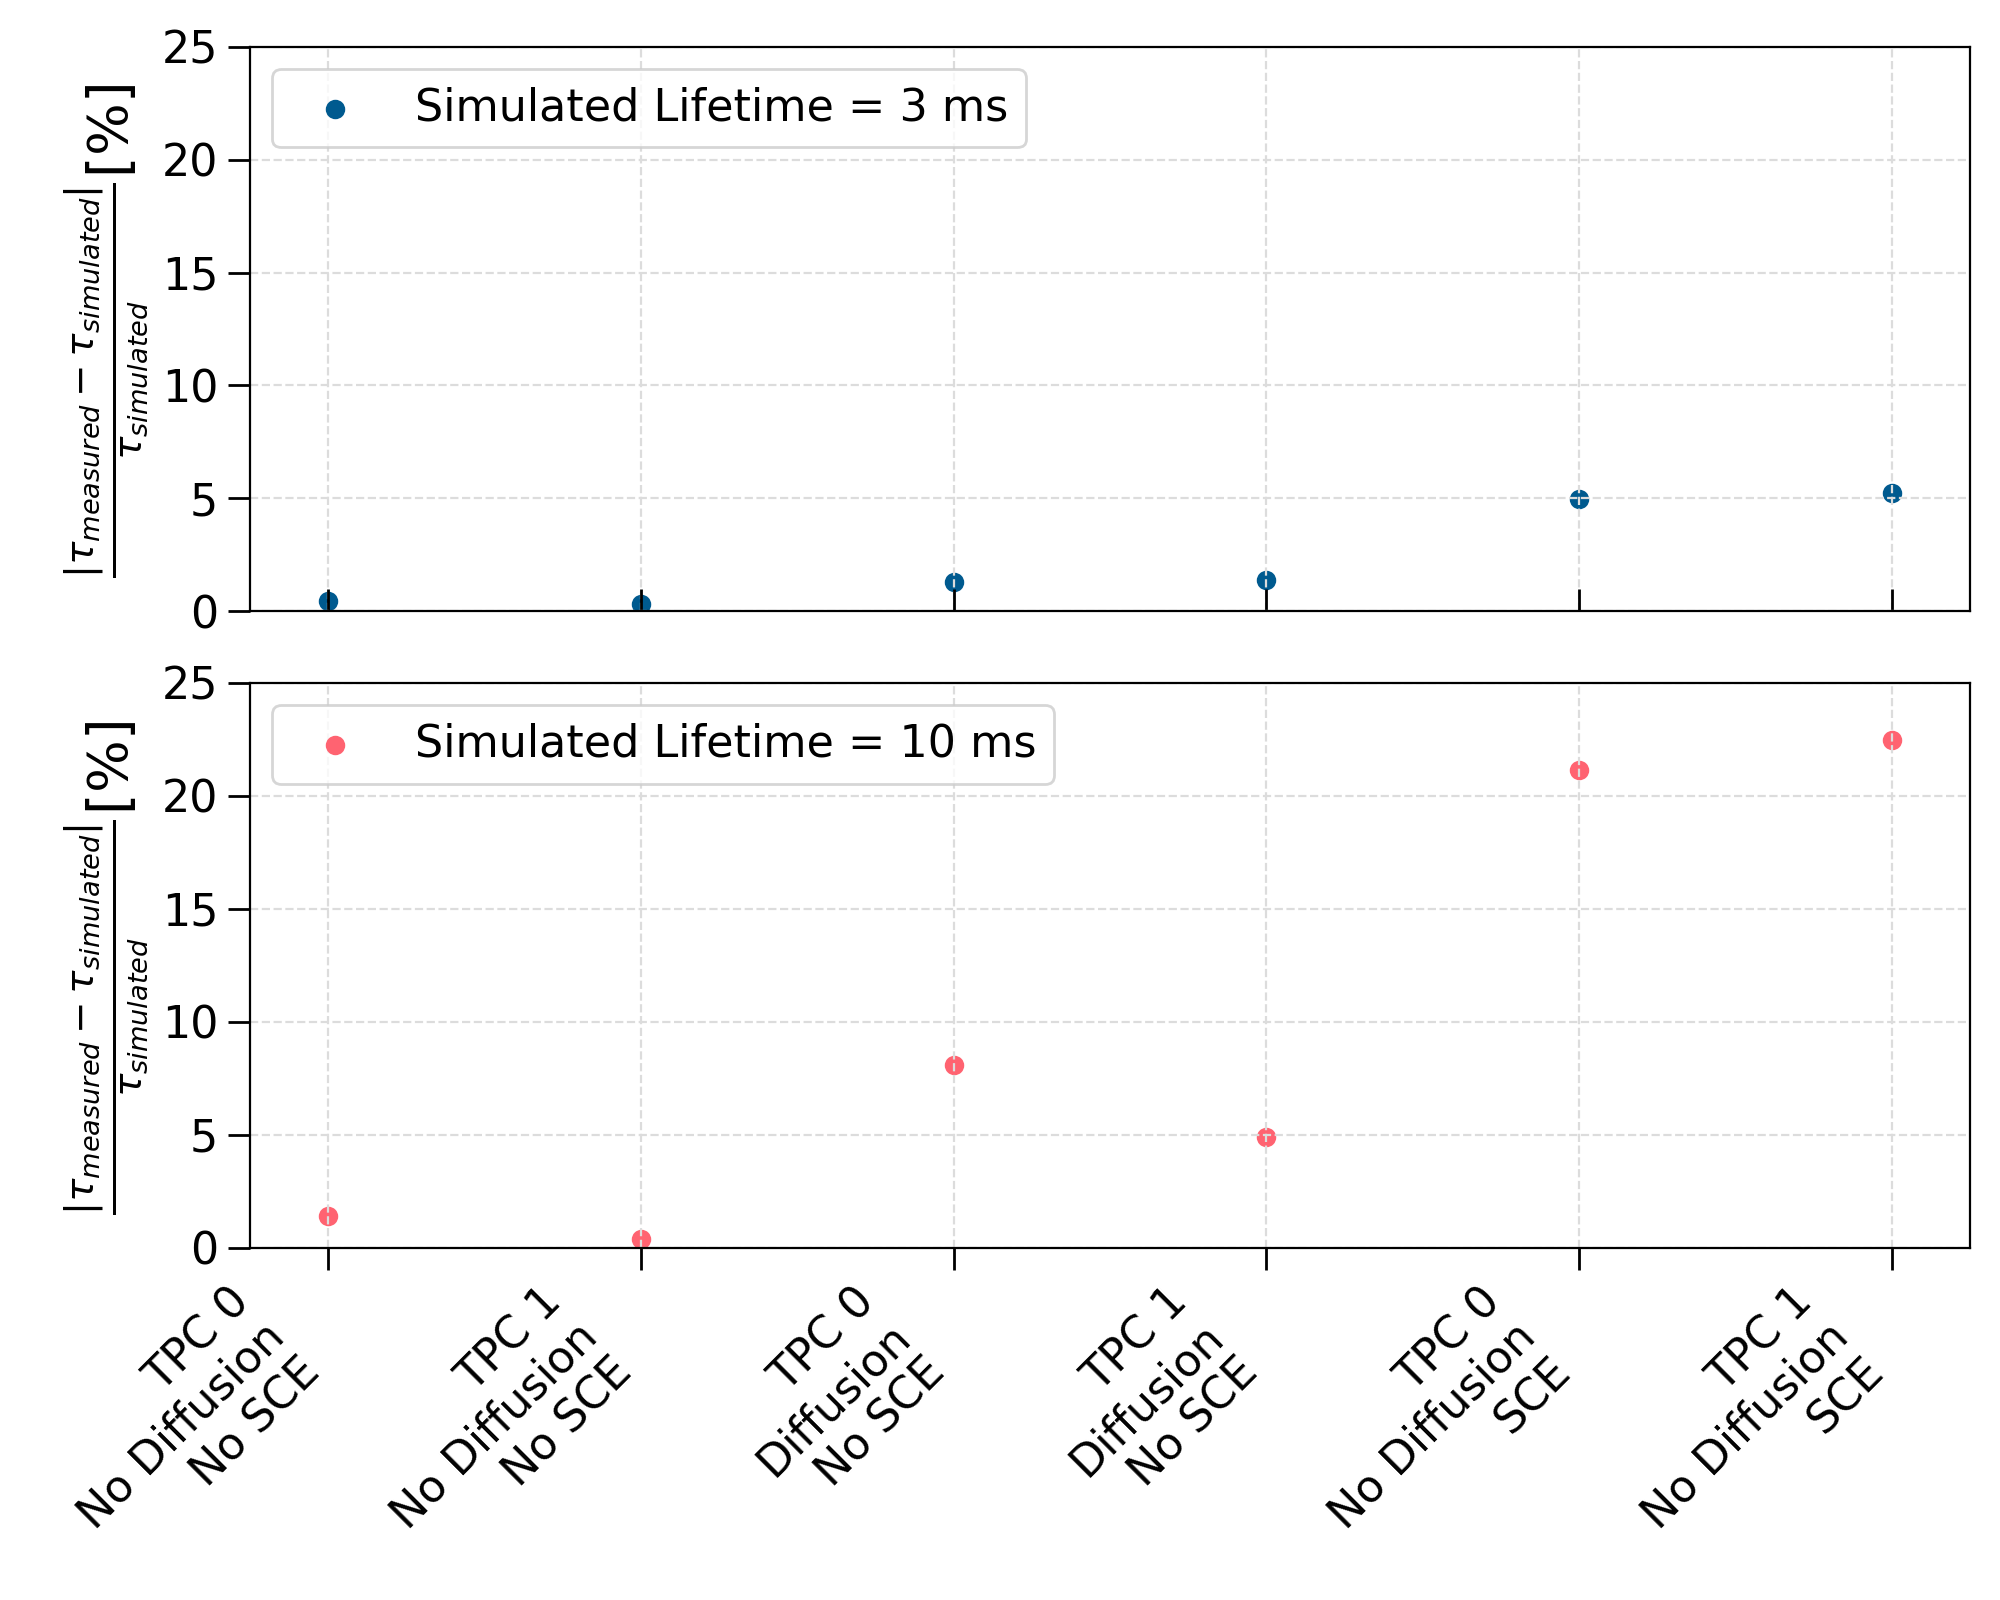
\includegraphics[width=0.75\textwidth]{etime_biases_compare}
\caption[etime_biases_compare]{
Biases in measured electron lifetimes compared to simulated values, due to diffusion and space charge effects.
}
\label{fig:etime_biases_compare}
\end{figure}

Biases in the measured lifetime compared to the simulated lifetime are shown in Fig. \ref{fig:etime_biases_compare}, for two simulated electron lifetimes at 3 ms and 10 ms.
When neither diffusion nor SCE were enabled in the simulation, the measured lifetimes were unbiased compared to the simulated lifetimes.
At both simulated values of electron lifetimes, the observed biases are well below the 5\% level.
When either diffusion or SCE was enabled in the simulation, biases in the measured lifetimes can be seen.
The magnitude of the biases due to SCE is much greater than due to diffusion, which is consistent with the observations from an electron lifetime measurement carried out by MicroBooNE \cite{ubooneEtime}. 
The paper demonstrated that the traverse component of diffusion causes similar biases in the measured lifetime as SCE however, at a smaller magnitude.
The paper also pointed out that the longitudinal component of diffusion causes insignificant biases in the measured lifetime.
Moreover, the comparison between the two simulated lifetimes at 3 ms and 10 ms shows that the longer the lifetime, the larger the biases.
It could be due to more drifting electrons surviving with longer lifetimes and thus, becoming more susceptible to detector effects.

\subsection{Concluding Remarks}
\label{sec7:etime_remark}

%New model of diffusion
The study demonstrates a method to measure electron lifetime using a sample of anode-to-cathode crossing cosmic tracks, that have the advantage of spanning over a full drift distance and a reconstructable $t_{0}$ time when the particle enters the detector.
Furthermore, the bias study shows that the measured electron lifetime by this method is the most affected by SCE, followed by diffusion, which is consistent with the observed results from MicroBooNE.
This procedure has now been replicated in preparation for the calibration run of SBND in the summer of 2024, where a calibration trigger will be deployed to tag crossing tracks for lifetime measurement.

Since this simulated study was carried out in 2021, the understanding of detector effects on observed energy deposition in LArTPC, and consequently electron attenuation, has been greatly improved.
An investigation carried out by Putnam and Schmitz at the ICARUS experiment demonstrated that traverse diffusion breaks down the Landau MPV approximation \cite{GrayDiffusion} of measured charge.
The paper recommends using an averaged $dQ/dx$ from a group of wires instead of $dQ/dx$ from a single wire to mitigate the effect of traverse diffusion smearing charge deposition across multiple wires.
The suggestion has now been implemented in the calibration workflow of SBND.

%********************************** %First Section  **************************************

\section{Delta Ray Fluctuations on Recombination Simulation}
\label{sec7:delta}

%Introduce why this is important
As discussed in Chapter \ref{Chapter6}, simulation plays a vital role in neutrino physics.
The need to correctly simulate physics processes must be addressed to validate against data and build towards a data-driven simulation.
The physics process of this simulated study is recombination, which drives the charge and light yield.                                              
As described in Sec. \ref{sec:recomb}, the recombination model employed at SBND is a phenomenological model, with parameters that have been experimentally measured by ArgoNeuT and tuned for simulation to match data \cite{argoneut_recomb}.
The Modified Box (ModBox) model approximates the recombination probability based on a cylindrical column surrounding a track-like charge deposition.
This volume treatment effectively accounts for microphysics processes produced along the track, such as delta rays, as some additional charges of the track itself.
This approximation has proven to work well for the MeV to GeV-scale interactions, however, breaks down when applied to keV-scale interactions.
The NEST collaboration pointed out non-linear fluctuations in recombination at increasingly smaller scales, which is currently not well-described by the ModBox model \cite{NEST}.   
Moreover, the ArgoNeuT collaboration also proposed that microphysics effects could lead to disagreements in recombination theory, simulation and measurement \cite{argoneut_recomb}.

One microphysics process that can affect recombination, highlighted by both NEST and ArgoNeuT collaborations, is delta ray.
Delta rays are high $dE/dx$ knock-out electrons with energy as low as 1 keV.
As shown in Fig. \ref{fig:delta_ray_evd}, delta rays can be seen as short tracks produced along a longer primary track, in this case, a cosmic muon.                      
Since delta rays have high $dE/dx$, they are associated with a smaller recombination factor, producing more scintillation photons while quenching ionisation electrons.
This simulation investigation examines how fluctuation in delta rays impacts the recombination simulation, and consequently, the energy-charge scales of different particle types.
Sec. \ref{sec:simDeltaRay} explains the simulation framework of delta rays and recombination, and expresses some concerns with the current framework.
Sec. \ref{sec:impactDeltaRayMag}, \ref{sec:impactDeltaRaySmear} and \ref{sec:impactStepLimit} describe the impacts of varying simulation handles associated with delta rays on particle calorimetry.
Finally, Sec. \ref{sec:concludeDeltaRay} suggests recommendations for measurements at SBND to improve the recombination model.             
                                                                                                                       
\begin{figure}[bp!] 
\centering    
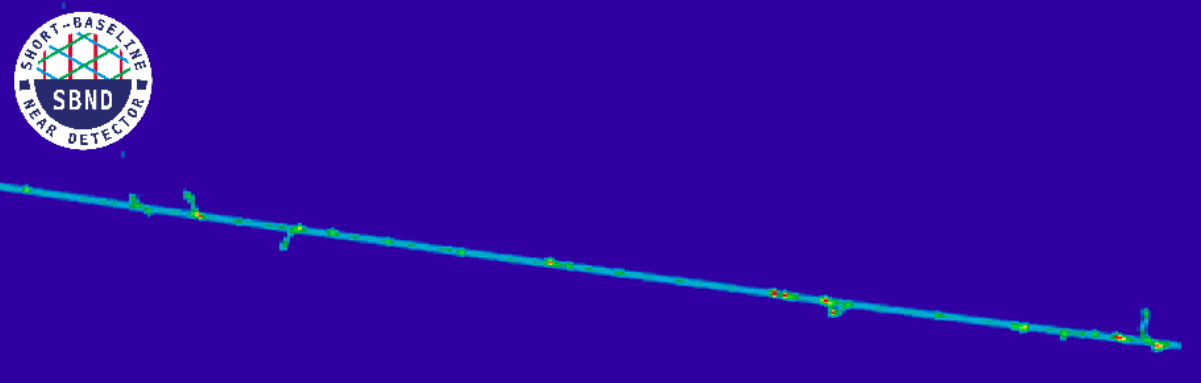
\includegraphics[width=0.85\textwidth]{delta_ray_evd}
\caption[delta_ray_evd]{
Event display of a simulated cosmic muon track segment, with many delta rays produced along the primary track.
}
\label{fig:delta_ray_evd}
\end{figure}


\subsection{Simulation of Delta Rays and Recombination}
\label{sec:simDeltaRay}

%Describe delta rays simulation
The physics of particle propagation from creation to detection point is simulated at the LArG4 stage.
This stage propagates the primary particle step by step and applies physics processes to each step of length $dx$.
LArG4 simulates the physics of energy loss due to ionisation as two intertwined processes: (1) a continuous energy loss $dE$ of the primary particle along the step $dx$ and (2) a discrete energy loss $dE$ at the end of the step producing delta rays \cite{geant4}.
The continuous energy loss of the primary particle is simulated by LArG4 using complementary models depending on the energy range and particle charge \cite{geant4_ions}.
The Bethe-Bloch formalism, detailed in Sec. \ref{sec3:bethebloch}, is used to compute $dE/dx$ in the high energy range (> 2 MeV), and the free electron gas model is applied at the low energy range (< 1 keV for protons).
In the intermediate range, parameterised models based on data from Ziegler \cite{Ziegler} and ICRU \cite{ICRU} are implemented.

Meanwhile, the total cross-section of the delta ray production is computed using a user-defined energy threshold.
The energy threshold defines the lower limit of the kinetic energy of the generated delta rays such that only delta rays with sufficient energy can be produced.
This is to suppress the generation and tracking of all low energy delta rays that would exhaust computation resources.
This also means that the energy of the non-produced delta rays is transferred to the continuous energy loss component of the primary particle.
This is equivalent to setting the energy threshold as the upper limit for the primary particle so that its mean energy loss is less than the threshold.
In other words, the energy threshold determines how much energy deposition is shared between the primary particle and the delta rays. 
The lower the threshold, the more energy deposition is carried away by the delta rays instead of the primary particle. 

In LArG4 terminology, this energy threshold is also known as the secondary production threshold, where the minimum kinetic energy requirement for delta ray production is defined as the minimum distance the generated delta ray must be able to traverse in a given material. 
For the standard simulation in SBND, the secondary production threshold for delta rays in a LAr medium is set as 700 $\mu$m, equivalent to a delta ray having a kinetic energy of 273 keV.
%This also means that the secondary production threshold also limits the interaction length of delta rays with LAr. 
Moreover, the maximum length $dx$ that the particle can propagate per step is configured as 0.3 mm, one order of magnitude smaller than the wire pitch.
This setup allows for a more feasible computation of generating delta rays.

%Describe ionandscint module
Recombination is then simulated for each step to determine the charge and light yield.
SBND employs the ModBox model, describing the energy-charge scale as follows
\begin{equation}
	\label{eq:recomb_modbox}
	\frac{dE}{dx} = \frac{1}{\beta}\left[ \exp{\left( \beta W_{ion}  \frac{dQ}{dx}\right)} -\alpha \right]
\end{equation}
where $\alpha = 0.93\pm0.02$ and $\beta = 0.212\pm0.002$ (kV/cm)(g/cm$^{2}$)/MeV, which are parameters that have been experimentally derived by ArgoNeuT \cite{argoneut_recomb}.
Recombination is highly dependent on the electric field and the local charge density, and therefore a parameter for the electric field is folded into the $\beta$ parameter.
By re-arranging Eq. \ref{eq:recomb_modbox}, one can derive the formalism of the recombination factor $R$ as a function of $dE/dx$ as
\begin{equation}
	\label{eq:R_factor}
	R = \frac{\log{ \left( \alpha + \left(\beta \cdot dE/dx\right)/\varepsilon \right)}}{\left(\beta \cdot dE/dx\right)/\varepsilon} 
\end{equation}
where $\varepsilon$ is the electric field of the detector at the position of the step.
For each step $dx$, the number of electron-ion pairs is calculated by dividing the energy deposited $dE$ by the energy required to ionise an argon atom $W_{ion} = 23.6$ eV. 
Then, $R$ from in Eq. \ref{eq:R_factor} is applied to the number of electron-ion pairs according to the charge-light anti-correlation described by Eq. \ref{eq:Q} and \ref{eq:L}, to determine the final charge and light yield resulting from the step $dx$.

%potential issue
The parameters $\alpha$ and $\beta$ of Eq. \ref{eq:recomb_modbox} were measured by ArgoNeuT using a stopping proton sample, and wire planes with a pitch of 3 mm.
Thus, the simulation of delta rays and recombination can give rise to several concerns.                                                                                                       
The first concern is the assumption of a \textit{universal} recombination factor $R$.
The same value is applied to different types of ionising particles, which can influence the local ionisation density differently. 
Secondly, the secondary production threshold on delta rays removes low energy electrons in simulation, however, they are produced in reality and can fluctuate recombination at a local scale. 
The last concern is the step length $dx$ configured to be one order of magnitude smaller than the wire pitch of both ArgoNeuT and SBND, resulting in the effective recombination $R$ being applied at microscopic scale.                                                                                                                     

%how to validate
The simulation investigation was set up to address individual concerns as well as to better understand their impacts on recombination.    
A truth comparison was carried out on two identical samples of muons and protons, to investigate if recombination is particle-dependent.
The particles were generated with a fixed energy of 1 GeV, uniform in positional and angular distributions.
The LArG4 stage was configured such that the particle can only deposit energy via ionisation.
Then, charge-based calorimetry was performed by reconstructing deposited energy $dE/dx$ from deposited charge $dQ/dx$ using Eq. \ref{eq:recomb_modbox}.

\subsection{Impacts of Delta Ray Fluctuations On Recombination Magnitude}
\label{sec:impactDeltaRayMag}

Fluctuations in delta rays were examined at different values of the secondary production thresholds ranging from 700 $\mu$m to 1 $\mu$m.
This is equivalent to generating delta rays of minimum kinetic energy ranging from 273 keV to as low as 1 keV.
The energy-charge plots of $dQ/dx$ to $dE/dx$ for proton are shown in Fig. \ref{fig:proton_2d}, for the secondary production threshold at 700 $\mu$m and 1 $\mu$m.
The calorimetry is plotted for the proton residual range from 1 cm to 90 cm, which covers the full track length. 
The proton $dE/dx$ proton ranges from 2 MeV/cm to 18 MeV/cm, allowing for the examination of delta ray fluctuation impacts at both low and high spectrum of $dE/dx$. 
For the secondary production threshold of 700 um, shown in Fig. \ref{fig:proton_2d_700}, the calorimetry distribution precisely follows the ModBox model with the ArgoNeuT parameters.
Good agreement is expected since the standard simulation of SBND is similar to the described simulation framework by ArgoNeuT \cite{argoneut_recomb}: (1) the maximum step length $dx$ was restricted to be 0.3 mm and (2) the energy loss due to delta rays was not included in recombination.
  
\begin{figure}[htbp!]
        \centering
        \begin{subfigure}[b]{0.495\textwidth}
            \centering
            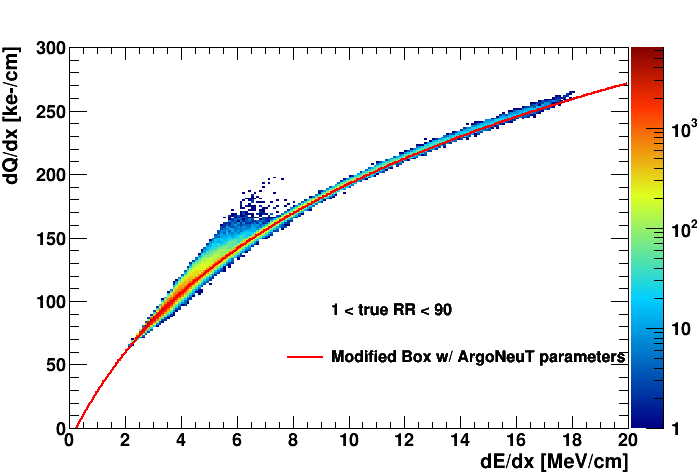
\includegraphics[width=\textwidth]{proton_700um}
            \caption{Secondary production threshold at 700 $\mu$m}%
            \label{fig:proton_2d_700}
        \end{subfigure}
        \hfill
        \begin{subfigure}[b]{0.495\textwidth}  
            \centering 
            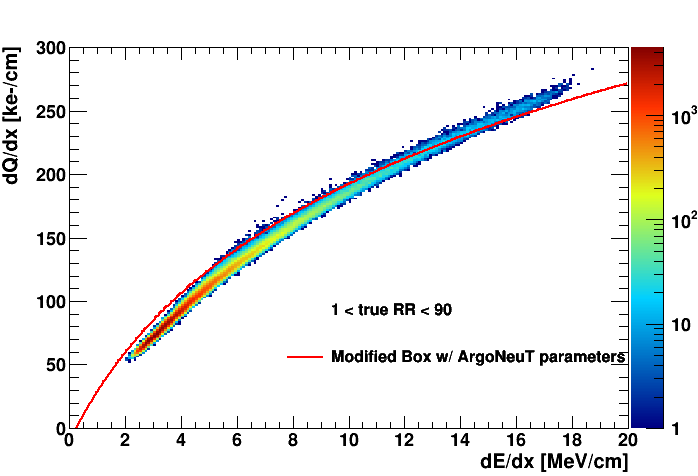
\includegraphics[width=\textwidth]{proton_1um}
            \caption{Secondary production threshold at 1 $\mu$m}%
            \label{fig:proton_2d_1}
        \end{subfigure}
        \caption{Plots of $dQ/dx$ as a function of $dE/dx$ for a 1 GeV proton at the secondary production threshold of 700 $\mu$m (left) and 1 $\mu$m (right)}
        \label{fig:proton_2d}
        %\vskip\baselineskip
\end{figure}

However, for the secondary production threshold of 1 um, shown in Fig. \ref{fig:proton_2d_1}, deviations away from the ModBox model occur, such that the energy-charge scale shifts in opposite directions at low $dE/dx$ compared to high $dE/dx$. 
Lowering the secondary production threshold leads to more energy deposition carried by the delta rays instead of the primary proton, and thus, delta rays have a greater influence on recombination.
At the low $dE/dx$ spectrum of the proton, delta rays have higher $dE/dx$ than that of the proton, resulting in the effective recombination factor being quenched. 
The opposite effect is seen at the high $dE/dx$ spectrum of the proton, resulting in the effective recombination factor increases.

%This then allows the determination of the output simulated recombination factor, given as $dE/dx / (W \times dQ/dx)$.
The energy-charge scale of proton at the secondary production thresholds at 700, 10, 5, and 1 $\mu$m, equivalent to delta rays with a minimum kinetic energy of 272.58, 14.60, 2.58, 1.06, and 0.99 keV are plotted in Fig. \ref{fig:proton_range_delta}. 
To compare $dQ/dx$ quantitatively at the same $dE/dx$ bin, the mean $dQ/dx$ is calculated per bin as shown in Fig. \ref{fig:proton_range_delta_magnitude}.
The percentage difference of the mean $dQ/dx$ relative to the ModBox model is plotted in Fig. \ref{fig:proton_range_delta_diff} to examine the magnitude of impacts from delta rays fluctuations on the energy-charge scale. 
Lowering the kinetic energy of delta rays results in two key trends.                                                           
Firstly, the $dE/dx$ position at which the proton energy-charge scale shifts in opposite directions, increases with lower delta ray kinetic energy. 
Secondly, the magnitude of the deviations is also dependent on the secondary production threshold, or the produced delta ray kinetic energy. 
At low $dE/dx$, the magnitude of the effective recombination quenching is the greatest for the secondary production threshold set as 1 $\mu$m. 
Meanwhile, at high $dE/dx$, the effective recombination is the highest for the secondary production threshold set as 10 $\mu$m. 
This is evident that delta ray fluctuations determine how much the proton is \textit{dressed} in delta rays, and can greatly influence the effective recombination factor across the $dE/dx$ spectrum of the proton. 
\begin{figure}[htbp!]
        \begin{subfigure}[b]{0.495\textwidth}   
            \centering 
            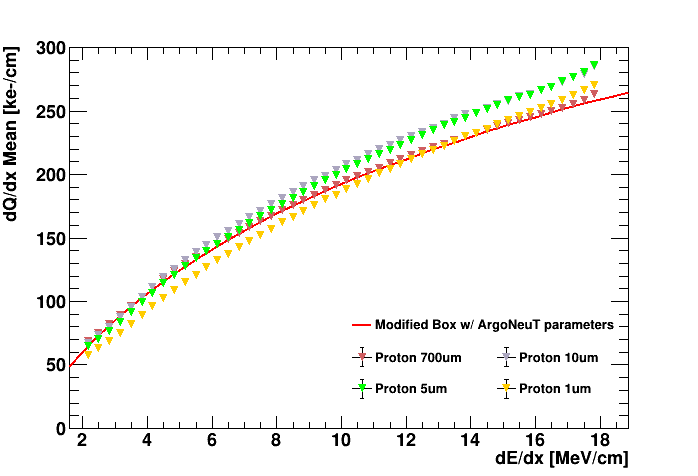
\includegraphics[width=\textwidth]{proton_profile}
            \caption{}%
            \label{fig:proton_range_delta_magnitude}
        \end{subfigure}
        \hfill
        \begin{subfigure}[b]{0.495\textwidth}   
            \centering 
            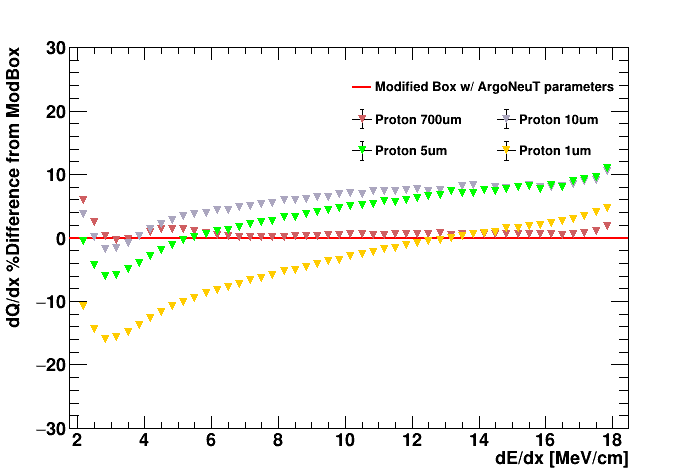
\includegraphics[width=\textwidth]{proton_profile_diff}
            \caption{}%
            \label{fig:proton_range_delta_diff}
        \end{subfigure}
        \caption{Plots of the mean $dQ/dx$ (left) and its percentage difference relative to the ModBox model (right) as a function of $dE/dx$ for a 1 GeV proton at various secondary production thresholds. }
        \label{fig:proton_range_delta}
\end{figure}

The calorimetry plot for muon is plotted in Fig. \ref{fig:muon_2d}, for the secondary production threshold at 700 $\mu$m and 1 $\mu$m respectively.
 Fig. \ref{fig:mu_2d_700} and \ref{fig:mu_2d_1} contain no restriction on the muon residual range, to fully cover the track length from 1 to 400 cm.
Two distinct distributions can be seen, one linear prong from the MIP region, and another one that follows the curve of the ModBox model indicating the stopping region. 
The linear energy-charge scale has been well-observed experimentally with MIP muons \cite{uboone_calib}.
%The linear distribution is due to the dressing the primary muon with very high energy delta rays, which have a linear energy-charge scale. 
%This result in this linear feature that has been well observed experimentally with MIP muons. 
To examine the stopping region exclusively, a residual range requirement of less than 10 cm is applied, as shown in Fig. \ref{fig:mu_2d_700_lowRR} and \ref{fig:mu_2d_1_lowRR}.
Some remnants of the MIP muon distribution can still be seen in the $dE/dx$ range between 4 to 12 MeV/cm.
Similarly to proton at the low $dE/dx$ scale, delta rays with lower kinetic energy result in quenching the effective recombination factor.
The mean $dQ/dx$ of muon and its percentage difference relative to the ModBox model are also plotted as shown in Fig. \ref{fig:mu_range_delta}.
The same behaviour as proton is observed such that the magnitude of the effective recombination quenching increases with lower delta ray kinetic energy.
Nonetheless, the magnitude of the quenching is larger for muon compared to proton.
The difference is driven by how each particle type is \textit{dressed} in a different amount of delta rays even at the same simulation configuration for delta rays.

\begin{figure}[htbp!]
        \centering
        \begin{subfigure}[b]{0.495\textwidth}
            \centering
            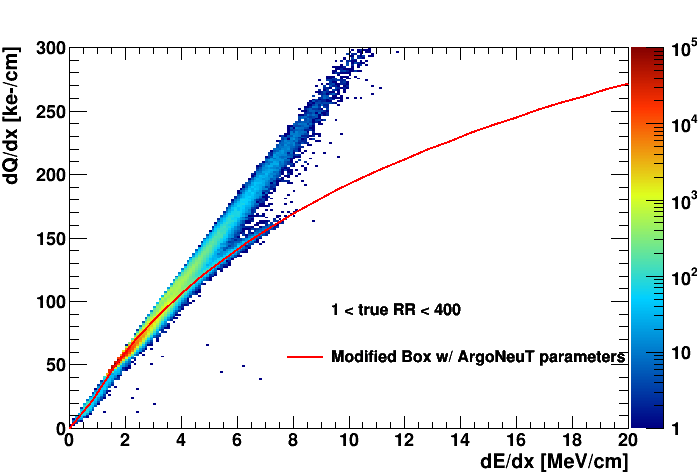
\includegraphics[width=\textwidth]{mu_700um}
            \caption{Secondary production threshold at 700 $\mu$m and full residual range}%
            \label{fig:mu_2d_700}
        \end{subfigure}
        \hfill
        \begin{subfigure}[b]{0.495\textwidth}  
            \centering 
            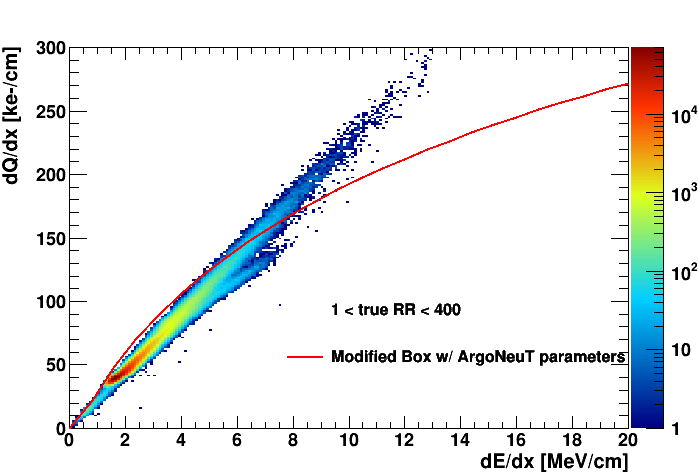
\includegraphics[width=\textwidth]{mu_1um}
            \caption{Secondary production threshold at 1 $\mu$m and full residual range}%
            \label{fig:mu_2d_1}
        \end{subfigure}
        %\vskip\baselineskip
        \begin{subfigure}[b]{0.495\textwidth}   
            \centering 
            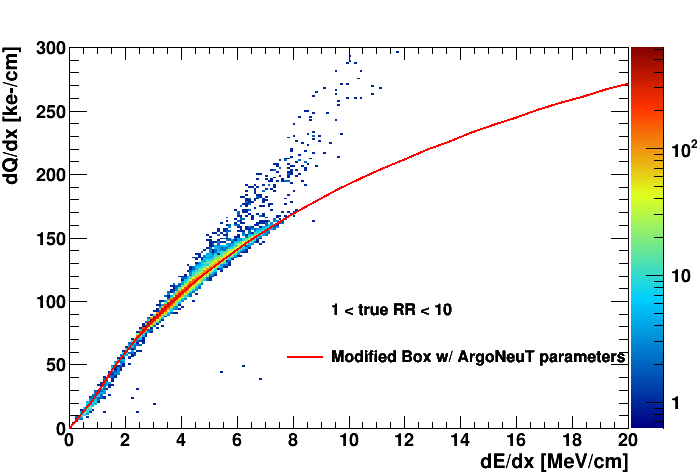
\includegraphics[width=\textwidth]{mu_700um_lowRR}
            \caption{Secondary production threshold at 700 $\mu$m and only stopping range}%
            \label{fig:mu_2d_700_lowRR}
        \end{subfigure}
        \hfill
        \begin{subfigure}[b]{0.495\textwidth}   
            \centering 
            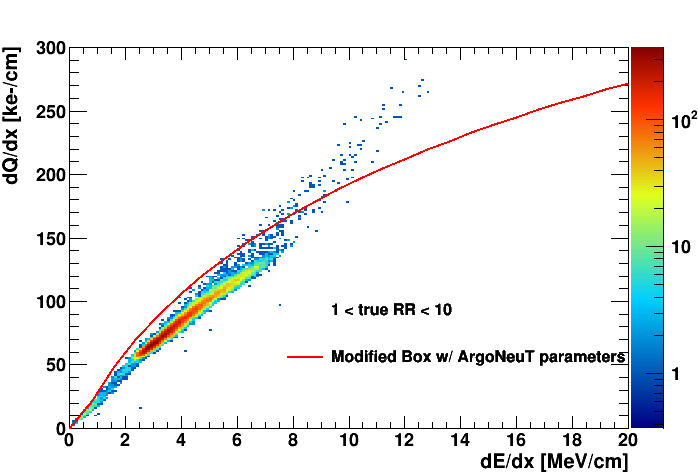
\includegraphics[width=\textwidth]{mu_1um_lowRR}
            \caption{Secondary production threshold at 1 $\mu$m and only stopping range}%
            \label{fig:mu_2d_1_lowRR}
        \end{subfigure}
        \caption{
        	Plots of $dQ/dx$ as a function of $dE/dx$ for a 1 GeV muon at the secondary production threshold of 700 $\mu$m (left) and 1 $\mu$m (right).
		Full residual range of the muon is included in the top plots and only stopping range is included in the bottom plots.
	}
        \label{fig:muon_2d}
\end{figure}
\begin{figure}[htbp!]
        \begin{subfigure}[b]{0.495\textwidth}   
            \centering 
            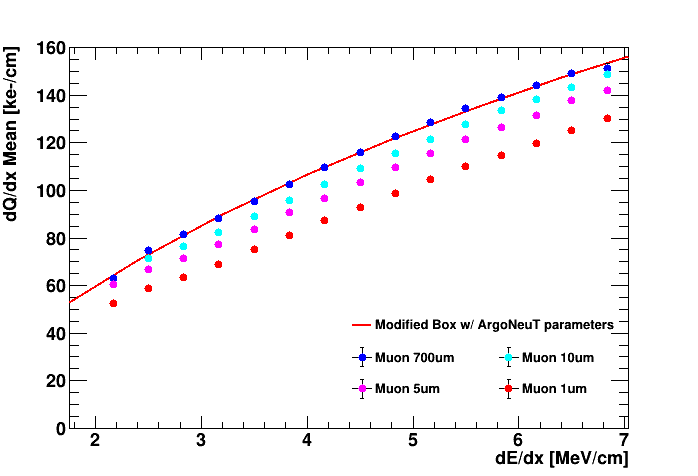
\includegraphics[width=\textwidth]{mu_profile}
            \caption{}%
            \label{fig:mu_range_delta_magnitude}
        \end{subfigure}
        \hfill
        \begin{subfigure}[b]{0.495\textwidth}   
            \centering 
            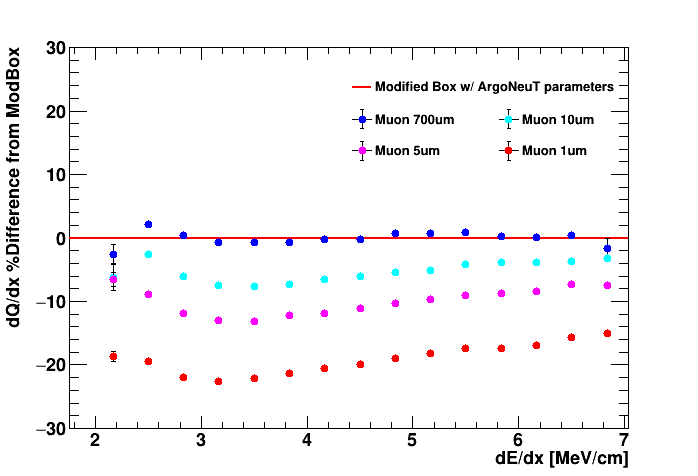
\includegraphics[width=\textwidth]{mu_profile_diff}
            \caption{}%
            \label{fig:mu_range_delta_diff}
        \end{subfigure}
        \caption{Plots of the mean $dQ/dx$ (left) and its percentage difference relative to the ModBox model (right) as a function of $dE/dx$ for a 1 GeV muon at various secondary production thresholds. }
        \label{fig:mu_range_delta}
\end{figure}

\subsection{Impacts of Delta Ray Fluctuations On Recombination Smearing}
\label{sec:impactDeltaRaySmear}

The effects of delta rays on recombination also extend to smearing of the energy-charge scale.
To de-tangle how the LArG4 simulation framework handles the smearing due to delta rays, an additional study was carried out by isolating only the energy deposition of the primary particle.
Fig. \ref{fig:proton_derr} shows the $dE/dx$ of the primary proton as a function of its residual range, compared against the Landau-Vavilov distribution \cite{Passage}.
Energy loss due to delta rays is included in the top two plots, Fig. \ref{fig:derr_proton_delta_700} and Fig. \ref{fig:derr_proton_delta_1}, for the secondary production thresholds of 700 $\mu$m and 1 $\mu$m.
Meanwhile, the bottom two plots, Fig. \ref{fig:derr_proton_only_700} and Fig. \ref{fig:derr_proton_only_1}, only include the energy loss of the primary proton.
The same set of plots are also computed for the case of muon as shown in Fig. \ref{fig:mu_derr}.

When delta rays are included in the energy deposition, the $dE/dx$ distribution agrees with the Landau-Vavilov distribution with smearing in $dE/dx$ across all bins of the residual range.
The distributions are indistinguishable between the secondary production threshold at the default secondary production threshold of 700 $\mu$m and 1 $\mu$m, comparing Fig. \ref{fig:derr_proton_delta_700} and Fig. \ref{fig:derr_proton_delta_1} for proton and comparing Fig. \ref{fig:derr_mu_delta_700} and \ref{fig:derr_mu_delta_1} for muon. 
The behavior is expected since the total energy deposition of the primary particle and the delta rays stay the same at different values of the secondary production threshold.
Comparing between the case of proton and muon, including delta rays in the energy deposition introduces greater smearing in the $dE/dx$ distribution for muon than that of proton.

For the secondary production threshold of 700 $\mu$m, the $dE/dx$ distribution of only the primary particle follows closely the Landau-Vavilov distribution, however with less smearing in $dE/dx$ compared to when delta rays are included in the energy loss.
This can be seen comparing Fig. \ref{fig:derr_proton_delta_700} and Fig. \ref{fig:derr_proton_only_700} for proton, and comparing Fig. \ref{fig:derr_mu_delta_700} and \ref{fig:derr_mu_only_700} for muon. 
The majority of the energy deposition is carried away by the primary particle, and LArG4 already accounts for fluctuations when sampling the mean energy loss of the primary particle.
Introducing delta rays only adds some additional smearing to the $dE/dx$ distribution.
%As stated previously, the secondary production threshold changes how much the energy loss is shared between the primary particle and the associated delta rays.
%This is evident when considering only the energy deposition of from the primary particle. 
\begin{figure}[tbp!]
        \begin{subfigure}[b]{0.495\textwidth}   
            \centering 
            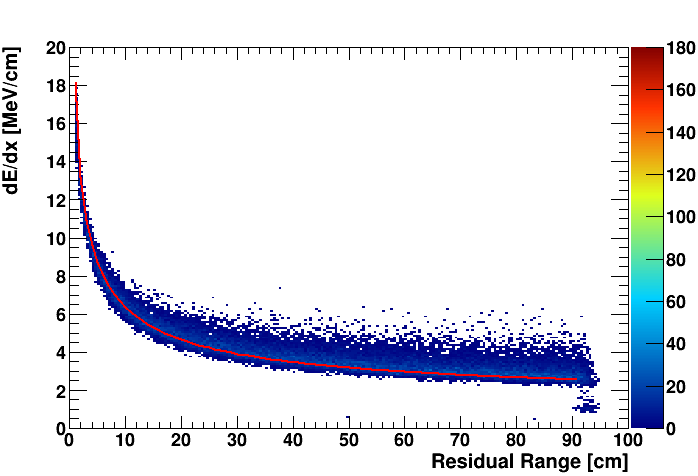
\includegraphics[width=\textwidth]{derr_proton_delta_700um}
            \caption{Secondary production threshold at 700 $\mu$m and delta rays are included}%
            \label{fig:derr_proton_delta_700}
        \end{subfigure}
        \hfill
        \begin{subfigure}[b]{0.495\textwidth}   
            \centering 
            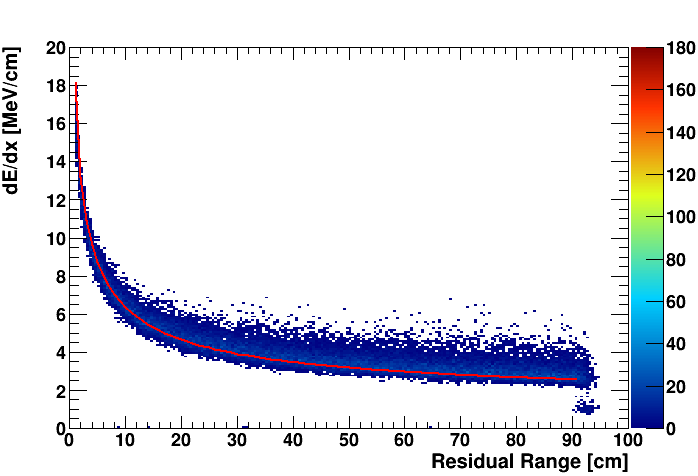
\includegraphics[width=\textwidth]{derr_proton_delta_1um}
            \caption{Secondary production threshold at 1 $\mu$m and delta rays are included}%
            \label{fig:derr_proton_delta_1}
        \end{subfigure}
        \begin{subfigure}[b]{0.495\textwidth}   
            \centering 
            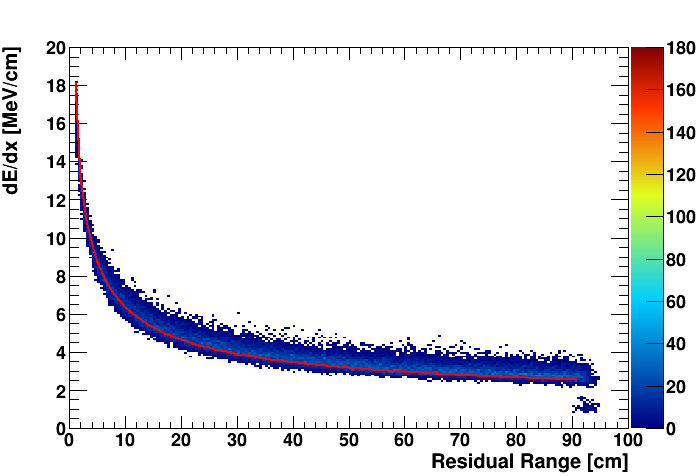
\includegraphics[width=\textwidth]{derr_proton_only_700um}
            \caption{Secondary production threshold at 700 $\mu$m and delta rays are excluded}%
            \label{fig:derr_proton_only_700}
        \end{subfigure}
        \hfill
        \begin{subfigure}[b]{0.495\textwidth}   
            \centering 
            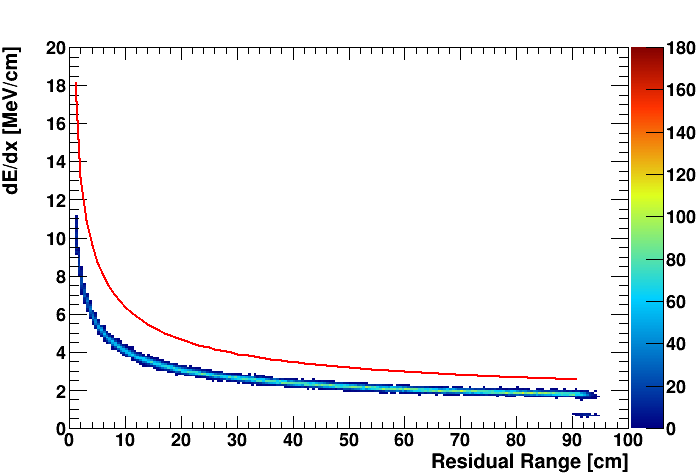
\includegraphics[width=\textwidth]{derr_proton_only_1um}
            \caption{Secondary production threshold at 1 $\mu$m and delta rays are excluded}%
            \label{fig:derr_proton_only_1}
        \end{subfigure}
        \caption{
	Plots of $dE/dx$ as a function of residual range for a 1 GeV proton at the secondary production threshold of 700 $\mu$m (left) and 1 $\mu$m (right). 
	The top (bottom) plots include (exclude) the energy loss due to delta rays. 
	}
        \label{fig:proton_derr}
\end{figure}

Meanwhile, when the secondary production threshold is set to 1 um and no delta rays are considered, the $dE/dx$ distribution of only the primary particle becomes narrow without any smearing and fails to follow the Landau-Vavilov distribution, which can be seen in Fig. \ref{fig:derr_proton_only_1} for proton and Fig. \ref{fig:derr_mu_only_1} for muon. 
Isolating only energy deposition of the primary particle is equivalent to observing a \textit{bare} proton or muon, such that the primary particle is not \textit{dressed} with any delta rays.
Experimentally, this has not been measured and therefore, the stopping power distribution of a \textit{bare} particle is computed by LArG4 by interpolation instead of using data-based parametrisation \cite{geant4}.
%On the other hand, when the secondary production threshold is configured at 1 $\mu$m, more energy loss is carried away by the delta rays. 
%The rest of the energy loss and smearing is compensated by the production of delta rays.

\begin{figure}[tbp!]
        \begin{subfigure}[b]{0.495\textwidth}   
            \centering 
            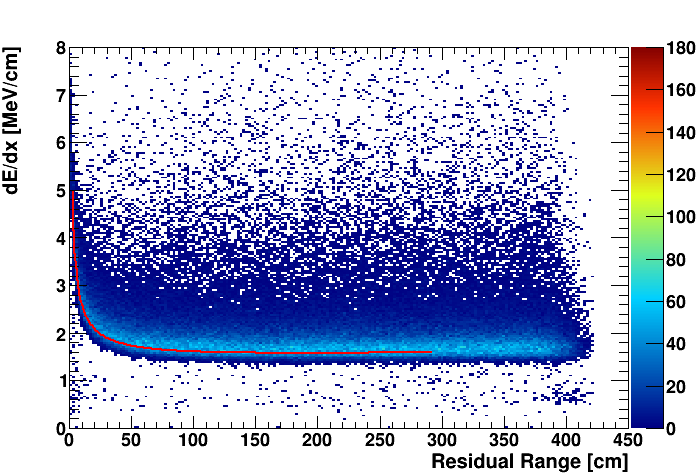
\includegraphics[width=\textwidth]{derr_mu_delta_700um}
            \caption{Secondary production threshold at 700 $\mu$m and delta rays are included}%
            \label{fig:derr_mu_delta_700}
        \end{subfigure}
        \hfill
        \begin{subfigure}[b]{0.495\textwidth}   
            \centering 
            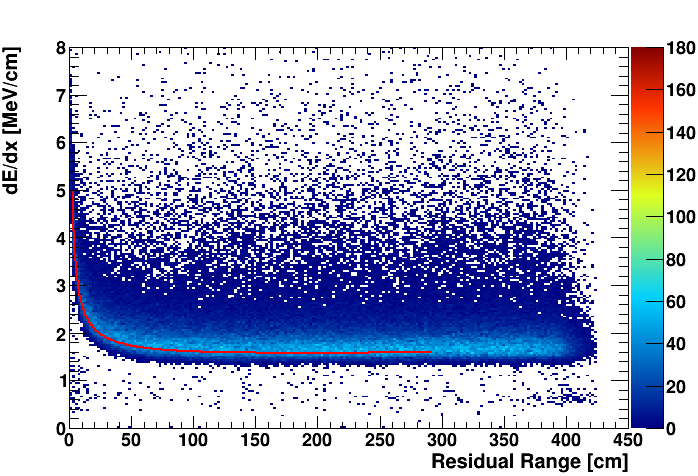
\includegraphics[width=\textwidth]{derr_mu_delta_1um}
            \caption{Secondary production threshold at 1 $\mu$m and delta rays are included}%
            \label{fig:derr_mu_delta_1}
        \end{subfigure}
        \begin{subfigure}[b]{0.495\textwidth}   
            \centering 
            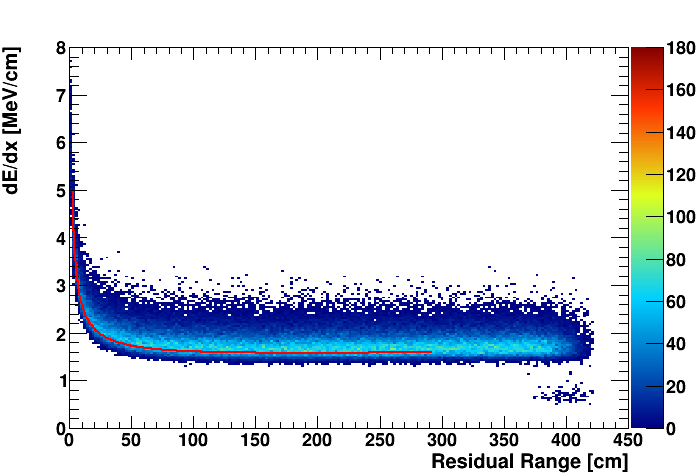
\includegraphics[width=\textwidth]{derr_mu_only_700um}
            \caption{Secondary production threshold at 700 $\mu$m and delta rays are excluded}%
            \label{fig:derr_mu_only_700}
        \end{subfigure}
        \hfill
        \begin{subfigure}[b]{0.495\textwidth}   
            \centering 
            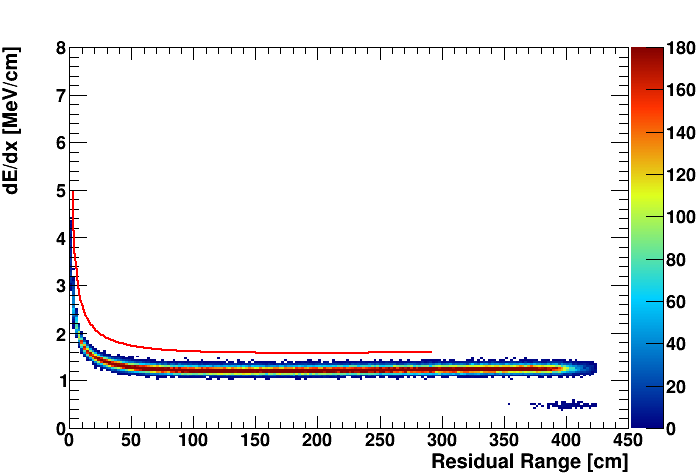
\includegraphics[width=\textwidth]{derr_mu_only_1um}
            \caption{Secondary production threshold at 1 $\mu$m and delta rays are excluded}%
            \label{fig:derr_mu_only_1}
        \end{subfigure}
        \caption{
	Plots of $dE/dx$ as a function of residual range for a 1 GeV muon at the secondary production threshold of 700 $\mu$m (left) and 1 $\mu$m (right). 
	The top (bottom) plots include (exclude) the energy loss due to delta rays. 
	}
        \label{fig:mu_derr}
\end{figure}

The simulated studies demonstrate that fluctuations of delta rays can introduce two different effects to recombination.
Firstly, delta rays have a different $dE/dx$ compared to the primary particle and therefore, influence the effective recombination factor.
At the low $dE/dx$ spectrum of the primary particle, this results in a significant quenching of recombination meanwhile at the high end of the $dE/dx$ spectrum, this can increase the observed recombination.
Secondly, having a different $dE/dx$ to the primary particle also means that delta rays can also smear the observed energy-charge scale.
Finally, the magnitude of the quenching and smearing effects vary between proton and muon, suggesting a need for a particle-dependent recombination factor.   

\subsection{Impacts of Step Limits}
\label{sec:impactStepLimit}
%Varying step limits and the effects on protons/muons

The step limit study here aims to investigate the impacts of simulating a phenomenological model at a microphysics scale.
The length $dx$, corresponding to the maximum distance the primary particle can travel per step, was studied at two configurable values: 0.3 mm and 3 mm.     
The former is the standard value employed in the simulation workflow of SBND as well as ArgoNeuT, which is one order of magnitude smaller than the wire pitch. 
The latter is the value of the wire pitch, which is the distance resolution observed by both detectors.

\begin{figure}[bp!]
        \begin{subfigure}[b]{0.495\textwidth}   
            \centering 
            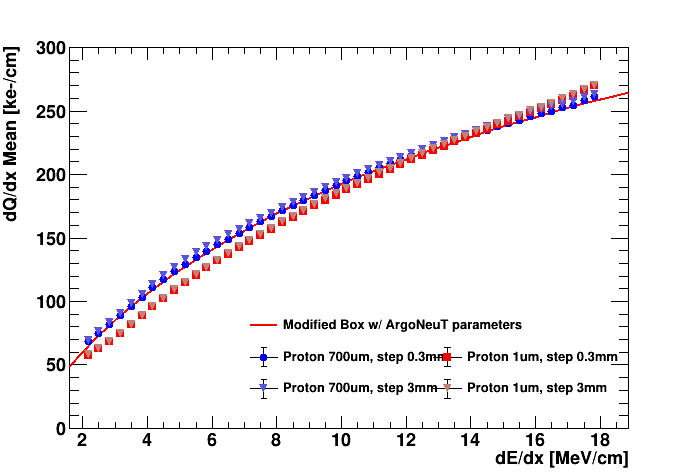
\includegraphics[width=\textwidth]{proton_profile_steplim}
            \caption{}%
            \label{fig:proton_steplim_magnitude}
        \end{subfigure}
        \hfill
        \begin{subfigure}[b]{0.495\textwidth}   
            \centering 
            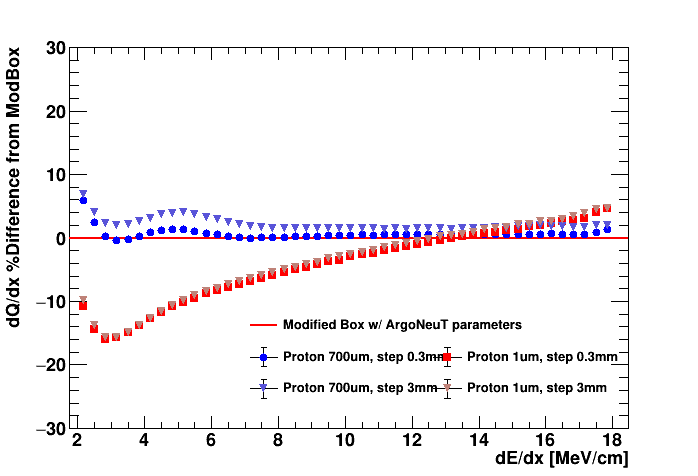
\includegraphics[width=\textwidth]{proton_profile_diff_steplim}
            \caption{}%
            \label{fig:proton_steplim_diff}
        \end{subfigure}
        \caption{Plots of the mean $dQ/dx$ (left) and its percentage difference relative to the ModBox model (right) as a function of $dE/dx$ for a 1 GeV proton, at secondary production thresholds of 700 $\mu$m and 1 $\mu$m and at step limits of 0.3 mm and 3 mm. }
        \label{fig:proton_steplim}
\end{figure}
A similar analysis using the energy-charge scale was employed.
The mean $dQ/dx$ as a function of $dE/dx$ for proton and its percentage difference to the ModBox model are plotted in Fig. \ref{fig:proton_steplim}, for different combinations of step limits, 0.3 mm and 3 mm, and of secondary production thresholds, 700 $\mu$m and 1 $\mu$m.
At the secondary production threshold of 700 $\mu$m, the increase of step limits from 0.3 to 3 mm results in an increase of the effective recombination factor across the whole range of $dE/dx$.
The largest magnitude of the increase is between the range $dE/dx$ from 2 to 8 MeV/cm, where the majority of energy deposition occurs, and reduces with a higher value of $dE/dx$. 
On the other hand, at the secondary production threshold of 1 $\mu$m, the effect of varying the step limit is insignificant.
The step limit increase affects the primary particle more than the delta rays.
This is due to the track length of the primary particle being significantly longer than that of delta rays, and therefore, more likely to propagate with a step length up to 3 mm.

This result demonstrates that even though the recombination model was simulated at the observed wire pitch distance of 3 mm, the resulting simulation does not return the input ModBox recombination model.
This is because the ArgoNeuT parameters were tuned using a simulation with the step length $dx$ configured at 0.3 mm.
Therefore, the simulation workflow of SBND likely only shows a good agreement when using the same configuration as ArgoNeuT.
This shows a strong inter-dependency between the detector simulation and experimental data, particularly when it comes to tuning a phenomenological parameter for a simulation workflow.

\subsection{Concluding Remarks}

\label{sec:concludeDeltaRay}

\begin{figure}[bp!]
\centering 
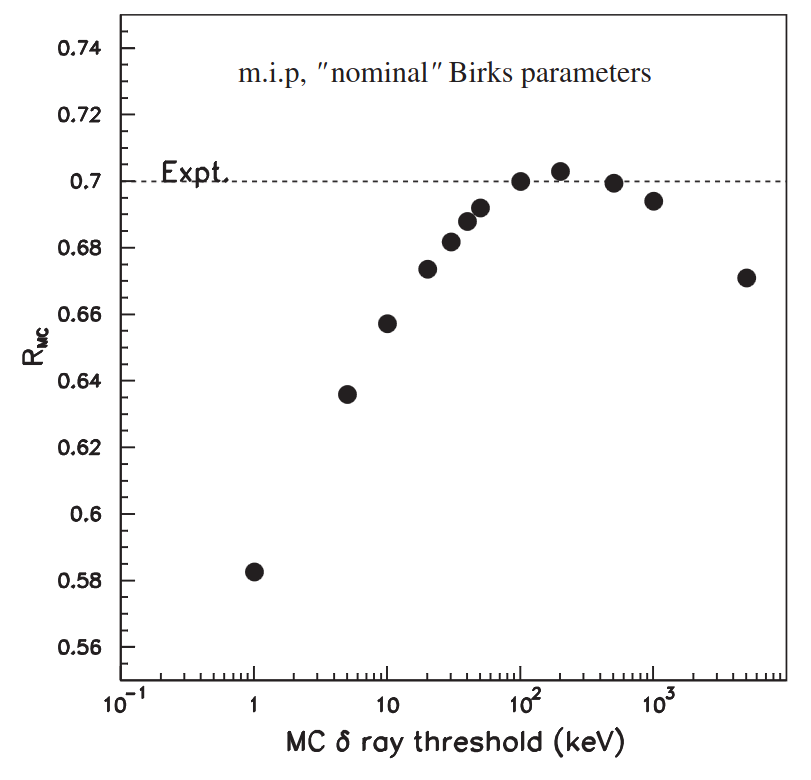
\includegraphics[width=0.5\textwidth]{icarus_recomb}
\caption{
The simulated recombination factor as a function of the secondary production threshold as carried out by the ICARUS collaboration.
The dotted line is the measured recombination factor using Birks formalism. 
Fig. from \cite{icarus_recomb}.
}
\label{fig:icarus_recomb}
\end{figure}

%ICARUS paper and why using 700 um
The simulated study shows that fluctuations in delta rays can influence the recombination factor.
A similar simulation-data comparison study of recombination was carried out by the ICARUS collaboration \cite{icarus_recomb}.
The result is shown in Fig. \ref{fig:icarus_recomb}, showing a quenching effect of the recombination factor at both low and high values of secondary production thresholds.
The experiment proposed a few different approaches toward recombination simulation.
The first approach is to simulate \textit{as microscopic as possible}, by generating low energy delta rays with kinetic energy as low as 1 eV and a range of order tens of nm, which was done in this study.
However, it was concluded this method would not work for the same reasons that have been verified in this study.
Firstly, the recombination measured in data is of a particle \textit{dressed} in delta rays, and secondly, limited computing resource constraints generating and tracking delta rays in that order of magnitude.
Another proposal was an empirical approach, by choosing the best secondary production threshold in simulation to reproduce the data.
This number was found to be 3 $\mu$m, equivalent to delta rays having a kinetic energy of 10 keV.


%gain more understanding in recombination : angular dependency
%TODO: add ref recombination dependence on angular
Since this simulated study was done in 2021, the understanding and modelling of recombination have been greatly improved.
Notably, recent results from the ICARUS experiment \cite{} have demonstrated a clear dependence of recombination on the angle of the ionising particle track to the drift electric field. 
An ellipsoid modified box model of recombination was proposed and able to describe the data across all measured angles. 
Nonetheless, there remains a lot of work to enhance our current understanding of recombination.
In the scope of calibrating the SBND detector, it is highly recommended to follow a data-driven approach such that the simulation should be tuned to best match the observed data, as it has been done by earlier experiments like ICARUS and ArgoNeuT.
This simulated study demonstrates a strong inter-dependency between detector simulation and data and therefore, the accuracy of the recombination factor can be improved by using parameters tuned to data measured by SBND.
Moreover, the study shows a distinct difference in recombination between proton and muon and perhaps suggests a need for a particle-dependent model.
Modelling recombination for a specific sample of particle type is feasible with the large statistics of SBND. 
This will allow for constructing a particle-dependent recombination factor that can be directly input into LArG4.
